\section*{Série 1 cap. 3 - 15}
Distribuição de Poisson $P(x = k) = \frac{e^{-\lambda}.\lambda^k}{k!}$
\subsection*{A)}
\begin{lstlisting}[mathescape]
$\lambda$ = 3
x = k = 4
P(4) = $\frac{e^{-3}.3^4}{4!}$
P(4) $\approx$ 0,1680
P(4) $\approx$ 16,8%
\end{lstlisting}
Código em R = dpois(4,lambda=3) \newline
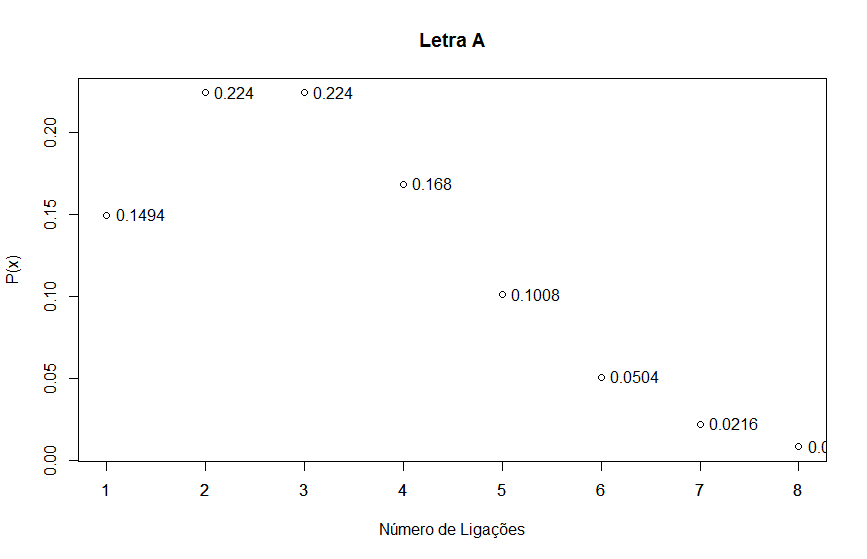
\includegraphics[width=\textwidth]{S1_15_A.png}


\subsection*{B)}
\begin{lstlisting}[mathescape]
P(x $\geq$ 3) = 1 - (P(0) + P(1) + P(2))
$\lambda$ = 3
P(1) = $\frac{e^{-3}.3^0}{0!}$
P(0) = 0,049787068

P(1) = $\frac{e^{-3}.3^1}{1!}$
P(1) = 0,149361205

P(2) = $\frac{e^{-3}.3^2}{2!}$
P(2) = 0,224041807

P(x $\geq$ 3) = 1 - 0,049787068 - 0,149361205 - 0,224041807
P(x $\geq$ 3) $\approx$ 0,5768
P(x $\geq$ 3) $\approx$ 57,68%
\end{lstlisting}
Código em R = ppois(2,lambda=3, lower=FALSE)\newline
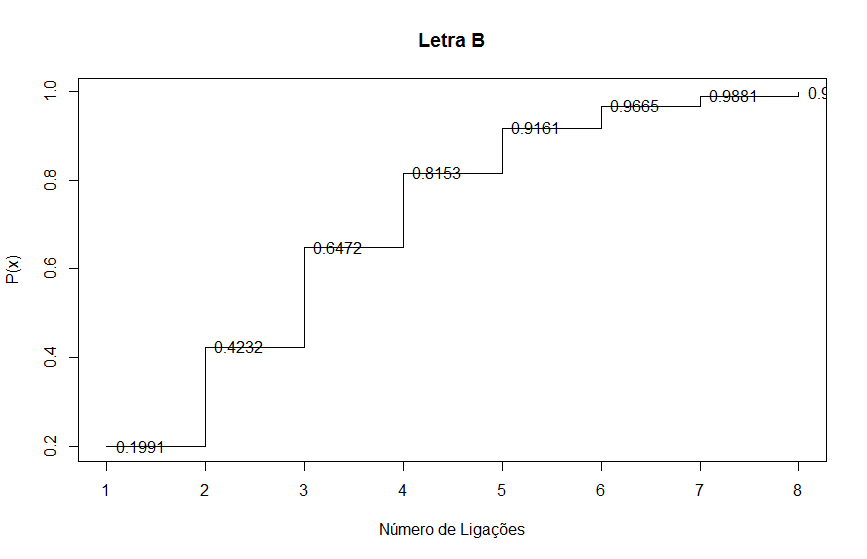
\includegraphics[width=\textwidth]{S1_15_B.png}